
\item A point travels along the \( x \) axis with a velocity whose projection \( v_x \) is presented as a function of time by the plot in Fig. 1.3.
    \begin{center}
        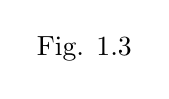
\begin{tikzpicture}
            % Since I cannot create the actual diagram, I'm placing a placeholder here.
            % You will need to replace this with the actual LaTeX/TikZ code for the diagram.
            \node at (0, 0) {Fig. 1.3};
        \end{tikzpicture}
    \end{center}
    Assuming the coordinate of the point \( x = 0 \) at the moment \( t = 0 \), draw the approximate time dependence plots for the acceleration \( w_x \), the \( x \) coordinate, and the distance covered \( s \).

\begin{solution}
    \begin{center}
        \begin{tikzpicture}
            \pic at (0, 0) {frame=3cm};
        \end{tikzpicture}
    \end{center}
    
    \begin{align*}
        \intertext{From question $v_x(0) = 0$, so the motion starts from origin, thus from the plot of $v_x(t)$ we have}
        v_x &= 
        \begin{cases} 
            0; & 0 \le t \le 1\\ 
            1; & 1 < t \le 3\\ 
            4-t; & 3 < t \le 6\\ 
            2t - 14; & 6 < t \le 7 
        \end{cases}
        \intertext{and $v_x=0$ for $t>7$.}
        \intertext{As at $t=0$, $x=0$,}
        \intertext{So,}
        x(t) &= \int_{0}^{t} v_x dt = 
        \begin{cases} 
            \frac{t^2}{2}; & 0 \le t \le 1\\ 
            t - \frac{1}{2}; & 1 < t \le 3\\ 
            4t - \frac{t^2}{2} + 5; & 3 < t \le 6\\ 
            t^2 - 14t + 49; & 6 < t \le 7 
        \end{cases}
        \intertext{Now,}
        s(t) &= \int_{0}^{t} |v_x|dt = 
        \begin{cases} 
            \frac{t^2}{2}; & 0 \le t \le 1\\ 
            t - \frac{1}{2}; & 1 < t \le 3\\ 
            4t - \frac{t^2}{2} - 5; & 3 < t \le 4\\ 
            \frac{t^2}{2} - 4t + 11; & 4 < t \le 6\\ 
            14t - t^2 - 43; & 6 < t \le 7 
        \end{cases}
        \intertext{Now,}
        a_x = \frac{dv_x}{dt} &= 
        \begin{cases} 
            1; & 0 \le t < 1\\ 
            0; & 1 < t < 3\\ 
            -1; & 3 < t < 6\\ 
            2; & 6 < t \le 7 
        \end{cases}
    \end{align*}
\end{solution}
